% Chapter Template

\chapter{Wood fracture behaviour under environment effects}
\label{Chapter1}

%----------------------------------------------------------------------------------------
%	SECTION 1
%----------------------------------------------------------------------------------------

\section{Wood behavior}


Wood is a living material which can be analyzed at different scales. Macroscopic and micrscopic scales are both, really important in order to understand wood behavior.

%-----------------------------------
%	SUBSECTION 1
%-----------------------------------
\subsection{Wood Structure and composition}

In macroscopic scale, wood material is composed of several parts. the first one, the heartwood, is the one with the best mechanical properties. It is considered as the dead part of wood which have a darkest colour than the other parts. It is the most used part of the tree for building utilisation. That is why, our specimen are made of it. Then, there is the sapwood, a living part of the wood, where the sap circulates. Heartwood is an older sapwood. Around the sapwood, there is the cambium. This part can evolute into sapwood or into the next layer, the bark. All these layers constitute a material which adapts is growth according to the constraints of its environment. That is one explanation of this study choice, which is based on wood analysis.

Microscopic scale show that, heartwood and sapwood are composed of tracheids and vessels linked by parenchyma. They are tubular component of the wood \ref{fig:Fig1}. They are composed of cellulose, lignin, and hemicellulose, which is the link between both type of cells \parencite{Reference1}.
\begin{figure}[th]
	\centering
	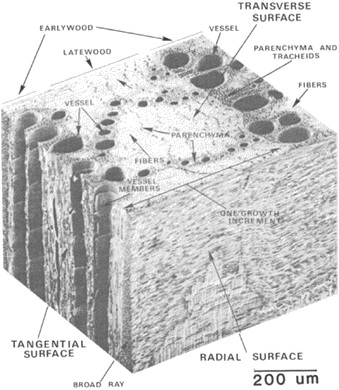
\includegraphics{Figures/Tracheids}
	\decoRule
	\caption[Wood microscopic composition]{Wood microscopic composition, presenting tracheids and vessels}
	\label{fig:Fig1}
\end{figure}
Tracheids allow to transport raw sap (from the ground, to the tree ramification) and elaborated sap (from the ramification to the ground). Some vessels are also perpendicular to wood grain. A phenomenon of capillarity explain how sap can circulate into vessels and tracheids. It is also explained by vegetative transpiration, due to photosynthesis and allow sap movement too \parencite{Reference1}.

Cambium has the role of cellular division \parencite{Reference4} presents it, in his document. Cambium will divide in two different cells. Phloem which is the component of the bark, and xylem which is the cell of sapwood.  All these cells are composed of polymers as cellulose, lignin, and hemicellulose. These cells by their configuration (as the crystal one) are as resistant as steal. Lignin has different interest like the waterproofing on the cells’ walls. 
Wood is a material which has a specific behaviour due to the change of the relative humidity of the middle. This behaviour explains that norms forbid its utilisation when its internal moisture content exceeds 20\%. Indeed, due to the microscopic properties, it appears that the tracheids expands with moisture content increase. Water present into tracheids and vessels, make it inflated which involve a displacement. On the contrary, when the temperature increase, and relative humidity decrease, tracheids contain less water and retract, but it also involves a displacement. This phenomenon known as Shrinkage - Swelling have an important effect because of the radial and tangential stresses which occurs when all the tracheids expands while the wood is displacement blocked. 
Each wood has a percentage of humidity called saturation fiber point (SFP) which is approximately 30\% amount of water. Under that point, free water contains in tracheids, and vessels will evaporate, and the water contain in cellulose fibre will begin to evaporate too. This effect involve withdrawal. At the opposite, if the amount of water increases and exceed 30\%, there is swelling. 
To provide these effects, wood is often treated and dry before uses. But drying a wood element can produce cracks. When the wood is dry too fast, a located collapse of cells and a crack takes place. The objective in the drying process is to limit the amount of water to nearly 12\%. At its initial state, green wood is considered as a wood full of water. To prevent water effect, and have a 12\% relative humidity inside it, a heating process must be done. Examples can be the stove or a constant ventilation. Indeed, a natural dry will take one year, while an artificial one like, blowing constant hot and humid (at least 70\% of humidity) air, will take one month. 
These information allow to understand the experiments which will be done in this thesis work. But before presenting the experiments, some theoretical knowledges must be reminded. 


%----------------------------------------------------------------------------------------
%	SUBSECTION 2
%----------------------------------------------------------------------------------------

\subsection{An anisotropic and orthotropic material}

Wood is considered as an orthotropic material because the behaviour of its mechanical or thermal properties are not the same in its three mutually perpendicular directions. It is a particular anisotropy. This characteristic of the material can be explained by cellular arrangements, growth direction, and other biological elements \parencite{Reference1}. It involves mechanicals difference between each direction.
Wood has good mechanical characteristics. It is resistant in compression thanks to the strength of his structure. It is the same for traction resistance. However, this constate depend on the direction observed.  
The longitudinal direction presented on \ref{fig:Fig2}, is different than the others. Longitudinal direction is the one, which is the less impacted by water effects. Indeed, the tracheids swelling appears on the two others dimensions. So, it is a first independence of this direction on the others. Perpendicular plans, RL and RT are symmetrical. 
Therefore, regarding the tracheid constitution, it is trivial to understand that it is more resistant in term of traction or compression. Tracheid are composed, \parencite{Reference4} of solid polymers as cellulose or lignin. However, in the others direction, as tangential or radial one, a tracheid can be separated from the neighbour one, causing a crack due to the separation of tracheids. It is possible when the effort applied on the wood is a perpendicular (perpendicular from the longitudinal direction) traction one. That is why, tests are made on different surface.
\begin{figure}[th]
	\centering
	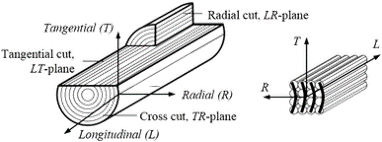
\includegraphics{Figures/Wood Surfaces}
	\decoRule
	\caption[Wood surfaces]{Wood surfaces depending on the direction}
	\label{fig:Fig2}
\end{figure}

%----------------------------------------------------------------------------------------
%	SECTION 2
%----------------------------------------------------------------------------------------

\section{Wood species}

Wood are separated into different species and two different groups: the temperate species and tropical species. The literature shows that the tropical species have better resistance due to this more complex microscopic structure characterized by its growth’s environment. This work present experiment on both type of wood. It is important to notice that hardwood (wood from leaves trees) and  softwood (wood from needles trees) have different behavior \parencite{Reference2}, but are presented in this work.

%----------------------------------------------------------------------------------------
%	SUBSECTION 1
%----------------------------------------------------------------------------------------

\subsection{Tropical species}

This work will focus on three tropical species, allowing to present woods with different density but from a same area, so dependant to same climatic constraints. Tropical types of woods are located in area, with an equatorial climate or humid tropical climate. Both are characterised by important rains. Equatorial climate has a constant and important pluviometry, while humid tropical climate is composed of a rainy season with torrential rains. Climate is one explanation of the growing differences between tropical and temperate species. In the case of this work, the study will be focused on three tropical species from Congo basin area (central Africa) in Gabon: Okume, Padouck and Iroko. All these species are hearthwood ones. 

Okoume specie (Aucoumea klaineana), has the smallest density. It is a wood present in central Africa. The major advantage of this specie is the speed of growth, which is one of the most impressive in wood world. According to CIRAD data \parencite{Reference5}, it has a circumference between 60cm to 120cm and can reach 50m high. The colour of this wood is composed of red nuances darkest depending on time. Rupture in compression occurs at a force of nearly 36MPa as \parencite{Reference5} present in Okoume wood sheet. It as a density of 0,44 which can be characterised as a light wood. It has a high SFP, equal to 40\% with a tangential withdrawal, superior to the radial one, and is in order of 6,9\%. For all this advantages, it is really used in construction, for carpentry, plywood, or shuttering panels. With a sapwood of approximately, 5cm, it allows to work with a large part of the three (heartwood principally). 

Padouck (Pterocarpus soyauxii Taub) is another tropical specie which has a bigger density, about 0,8 \parencite{Reference7}. It is considerate as a heavy wood. This characteristic explains its numerous uses in construction particularly. It can be used for bridge structure, carpentry, naval construction, plywood panels…   From 60cm to 100cm of diameter it also can reach 50m of high. It is less common and findable than Okoume specie. It must be dry, but it is an interesting wood in term of natural durability class (heartwood is classed in first durability class)
The Padouck is also a red nuances wood. It is one of the better compression resistance wood in the world, with a resistance until 70MPa. It has a SFP around 21\% and a tangential withdrawal of 5\%.

Iroko (Milicia excelsa) is the last wood presented. It is a compromised between the precedent species. It is not a red wood, but a yellow, brown one. It has visible tracheids and a density around 0,65 \parencite{Reference7} . It is also used for many usages, but not particularly construction. It can be used for parquet, woodworking, or cover plywood panels. One of the major advantages of this wood is the transformation of CO2 into calcium oxide crystals. It also considered as a viable wood considering insect and fungus resistance. It has a compression limit equal to 54MPa with an admit variation of 6MPa mentioned by the CIRAD. It has a tangential withdrawal double from the radial one, this value is 5,4\% and the SFP is 23\%.


%----------------------------------------------------------------------------------------
%	SUBSECTION 2
%----------------------------------------------------------------------------------------

\subsection{Temperate woods}

These trees are located in temperate area and are impacted by temperate climate. It is known that the temperate climate is characterised by four seasons and two important ones, the spring and summer. Indeed, during autumn and winter, trees are not growing waiting for rain and sun, which are essential for its expansion. In spring, the tree needs a lot of water and the cambium produce a large amount of sapwood. This sapwood made in spring is softer and quickly done at the contrary of summer sapwood, heavier with a bigger density. This thesis will compare the three species presented before with a European specie, the Silver Fir. It is a softwood from needles tree. 

The Silver Fir (Abies pectinata). Present on north hemisphere, it is a softwood as Pines or others old trees. As his name undertone, it has a white colour, and a circumference between 50 to 80cm. It has a density from 0,45 to 0.60 according to CIRAD data, a SFP about 30\% and a mechanical resistance in compression of 41MPa. The tangential withdrawal is important with a value of 8,7\%, while the radial withdrawal is 4\%. Thanks to it resistance it is used in carpentry, columns or light frame but must be treated against fungus and insects’ attacks. The main problem with this wood is the water bag contained into the tree. It also has problem of splitting which prevent uses of some connector in construction field.

%----------------------------------------------------------------------------------------
%	SUBSECTION 3
%----------------------------------------------------------------------------------------

\subsection{Explanation of this species choice and expected results}

The species presented were chosen among many others for different reasons. First, they have an interesting and different behavior. Indeed, they have different density but also mechanical behavior and are from different area and type of woods, as explained before. Then, there are really linked to the Civil ingeneering subeject. Except Okoume specie, all the other are not enough exploited for construction used. Gabon forest are composed of many wood, but without the use of some of them in construction field, as for Iroko and Padouck species. In France, the same fact appears in Massif Central forest, composed of many Silver Fir areas. By prooving that these species have a good comportement in humid environnemet, it could allow, their use in Construction field. Looking to \parencite{ref:Kif1998}, \parencite{ref:Ang2017}, \parencite{ref:Huang2020} works presenting wood behaviorr at different moisture content, or \parencite{ref:Seif2017} for diferent temperature, some values can be expected. Indeed, it is not the first work on this subject and our results could be discussed according to other articles.

\begin{table}[]
	\centering
	\begin{tabular}{cccc}
		\hline
		\rowcolor[HTML]{BFBFBF} 
		\multicolumn{1}{|c|}{\cellcolor[HTML]{BFBFBF}Reference} & \multicolumn{1}{c|}{\cellcolor[HTML]{BFBFBF}Specie} & \multicolumn{1}{c|}{\cellcolor[HTML]{BFBFBF}Climatical   Variation} & \multicolumn{1}{c|}{\cellcolor[HTML]{BFBFBF}Result} \\ \hline
		\multicolumn{1}{l}{} & \multicolumn{1}{l}{} & \multicolumn{1}{l}{} & \multicolumn{1}{l}{} \\ \hline
		\multicolumn{1}{|c|}{\cellcolor[HTML]{FFE699}\cite{Kif1998}} & \multicolumn{1}{c|}{Scots Pine} & \multicolumn{1}{c|}{Earlywood Green} & \multicolumn{1}{c|}{$\sigma$ = 49MPa} \\ \hline
		\multicolumn{1}{|c|}{\cellcolor[HTML]{FFE699}\cite{Kif1998}} & \multicolumn{1}{c|}{Scots Pine} & \multicolumn{1}{c|}{Latewood Green} & \multicolumn{1}{c|}{$\sigma$ = 74MPa} \\ \hline
		\multicolumn{1}{|c|}{\cellcolor[HTML]{FFE699}\cite{Kif1998}} & \multicolumn{1}{c|}{Scots Pine} & \multicolumn{1}{c|}{Earlywood resoaked} & \multicolumn{1}{c|}{$\sigma$ = 36MPa} \\ \hline
		\multicolumn{1}{|c|}{\cellcolor[HTML]{FFE699}\cite{Kif1998}} & \multicolumn{1}{c|}{Scots Pine} & \multicolumn{1}{c|}{Latewood resoaked} & \multicolumn{1}{c|}{$\sigma$ = 55MPa} \\ \hline
		\multicolumn{1}{|c|}{\cellcolor[HTML]{B4C6E7}\parencite{ref:Ang2017}} & \multicolumn{1}{c|}{Douglas Fir} & \multicolumn{1}{c|}{9\% MC} & \multicolumn{1}{c|}{$G_{max}$= 780J/$m^{2}$} \\ \hline
		\multicolumn{1}{|c|}{\cellcolor[HTML]{B4C6E7}\cite{Ang2017}} & \multicolumn{1}{c|}{Douglas Fir} & \multicolumn{1}{c|}{18\%MC} & \multicolumn{1}{c|}{$G_{max}$= 680J/$m^{2}$} \\ \hline
		\multicolumn{1}{|c|}{\cellcolor[HTML]{B4C6E7}\cite{Ang2017}} & \multicolumn{1}{c|}{White Fir} & \multicolumn{1}{c|}{9\% MC} & \multicolumn{1}{c|}{$G_{max}$= 580J/$m^{2}$} \\ \hline
		\multicolumn{1}{|c|}{\cellcolor[HTML]{B4C6E7}\cite{Ang2017}} & \multicolumn{1}{c|}{White Fir} & \multicolumn{1}{c|}{18\%MC} & \multicolumn{1}{c|}{$G_{max}$= 630J/$m^{2}$} \\ \hline
		\multicolumn{1}{|c|}{\cellcolor[HTML]{C6E0B4}\cite{Huang2020}} & \multicolumn{1}{c|}{Jack Pine} & \multicolumn{1}{c|}{2\% MC} & \multicolumn{1}{c|}{$\sigma$ = 4,5MPa} \\ \hline
		\multicolumn{1}{|c|}{\cellcolor[HTML]{C6E0B4}\cite{Huang2020}} & \multicolumn{1}{c|}{Jack Pine} & \multicolumn{1}{c|}{17\% MC} & \multicolumn{1}{c|}{$\sigma$ = 2,9MPa} \\ \hline
		\multicolumn{1}{|c|}{\cellcolor[HTML]{C6E0B4}\cite{Huang2020}} & \multicolumn{1}{c|}{Balsam Poplar} & \multicolumn{1}{c|}{2\% MC} & \multicolumn{1}{c|}{$\sigma$ = 5,4MPa} \\ \hline
		\multicolumn{1}{|c|}{\cellcolor[HTML]{C6E0B4}\cite{Huang2020}} & \multicolumn{1}{c|}{Balsam Poplar} & \multicolumn{1}{c|}{17\% MC} & \multicolumn{1}{c|}{$\sigma$ = 3,7MPa} \\ \hline
		\multicolumn{1}{|c|}{\cellcolor[HTML]{F4B084}\cite{Seif2017}} & \multicolumn{1}{c|}{Numerical} & \multicolumn{1}{c|}{-10 °C} & \multicolumn{1}{c|}{G = 8J/$m^{2}$} \\ \hline
		\multicolumn{1}{|c|}{\cellcolor[HTML]{F4B084}\cite{Seif2017}} & \multicolumn{1}{c|}{Numerical} & \multicolumn{1}{c|}{0 °C} & \multicolumn{1}{c|}{G = 9J/$m^{2}$} \\ \hline
		\multicolumn{1}{|c|}{\cellcolor[HTML]{F4B084}\cite{Seif2017}} & \multicolumn{1}{c|}{Numerical} & \multicolumn{1}{c|}{10 °C} & \multicolumn{1}{c|}{G = 11J/$m^{2}$} \\ \hline
	\end{tabular}
	\caption{Approximative results from previous works on climatical conditions affecting wood behavior.}
	\label{tab:ArticleResult}
\end{table}

So it is expected that with an increasement of the moisture content, the mechanical behavior must decrease, while by increasig the temperature of the specimen, the mechanical behavior should increase. However, this fact will also depends on the specie study.
Linked to the Moisture Content, if the temperature increase, there are less MC into the specimen, so it is expected that with a highter temperature, wood behavior should be better.

%-----------------------------------
%	SUBSECTION 3
%-----------------------------------

\subsection{Specimen geometry}

Many geometries can be used to allow experimental studies. This thesis choice is inspired on previous work and use MMCG specimen which derivate from DCB specimen which are rectangular piece of material. The purpose of MMCG specimen, \parencite{Reference6} is to involve a stable propagation of the crack in different mode and in mixed mode too. The study of this sample uses the rate of refund (G). G decrease while the crack is developing, until sample rupture. Tests on MMCG specimen can be study thanks to finite elements like the J integral method, which is used in this work. But also, by image analysis, like the DIC analysis.


\begin{figure}[th]
	\centering
	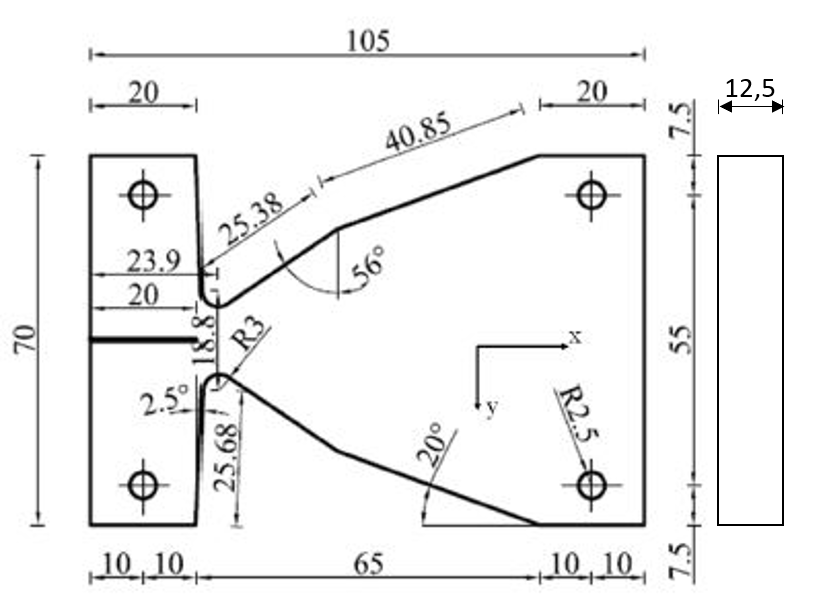
\includegraphics[scale=1.1]{Figures/MMCG_specimen}
	\decoRule
	\caption[MMCG specimen]{dimensions and geometry of Mixed Mode Crack Growth specimen}
	\label{fig:Fig5}
\end{figure}
MMCG sample is a compromise between DCB and CTS samples to obtain different mixing rates and a stable crack propagation. It is the specimen which will be used for this Development and Research Project, because of the good stability of the sample, presented in \parencite{Reference6} thesis. The Geometry, visible on \ref{fig:Fig5} was already tested in \parencite{Reference7} works. Manufactured samples of Okoume species with these dimensions were available in Polytech laboratory.

This work will focus on RL samples so Radial and Longitudinal surface. MMCG shapes are also linked to Compact Tension Shear (CTS) specimen. Indeed, the tiny dimensions of MMCG samples are similar to CTS ones. This geometry involves a little Fracture Process Zone (PFZ) which begin at the crack tip. But at the contrary of DCB specimen, the smaller dimensions of MMCG specimen does not allow a long displacement of the PFZ during the test. So after few minutes of displacement of the crack tip, the specimen will breack.

In mode one, a really progressive crack is expected. As it was said, \parencite{Reference6} developped this particular shape, to improve the stable propagation of the crack, more than in a DCB sample. Moreover, the different angles shown on \ref{fig:Fig5} and the rounded chamfer provide uncontrollable collapse of the specimen. Indeed, The optimization consists, on the variable inertia also used in DCB specimens. It was prooved by Finite Element Analysis (FEA) that the connection between the heels and the body of the specimen is a zone were strains are concentrated. These shapes allows By limiting the surface it avoids wood heterogenity. Beside, this compact geometry involves a faster increasement of the MC in the specimen. It is logical but can be remind by \ref{eq:moisture flux in wood}

\begin{equation}
	q_{m}= -\rho_{0}\cdot D \cdot \bigtriangledown m \\
	\\
	\left\{
	q_{m}: & moisture flux & \si{m^{3}/s} \\
	D: & Diffusivity & \si{m^{2}/s} \\
	\bigtriangledown: & Gradient & \\
	m: & moisture content & \% \\
	\right.
	
	\label{eq:moisture flux in wood}
\end{equation} 

body of the test tube and to strengthen its connection with the heels in order to concentrate the
breaking stresses, both in mode I and in mode II, at a crack point. Design
geometrical is thus carried out by finite elements.   
%----------------------------------------------------------------------------------------
%	SECTION 3
%----------------------------------------------------------------------------------------

\section{Rupture mechanics on wood}
Rupture mechanic has an objective to characterize the cracking behaviour of structures through stress field, crack size and cracking resistance of the material.

There are different rupture modes involve by the crack, the direction of the force which create the crack or compounds it. The first mode, called opening mode, characterized by a force applied, perpendicularly to the crack. The shearing mode is the second mode. The force is applied parallelly to the crack. And the third mode of rupture parallelly to the interior of the crack. The principals rupture mode are the first and the second, and this literature review will focus on first mode particularly. These modes are presented on \ref{fig:Fig3}. This first mode can be presenting by the energy release rate (G) linked to time or in our case, crack length, this plot is called R-curve.
\begin{figure}[th]
	\centering
	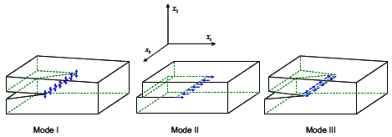
\includegraphics{Figures/Mode_presentation}
	\decoRule
	\caption[Crack modes]{Crack modes depending on the direction of the applied force.}
	\label{fig:Fig3}
\end{figure}
Four zones characterized this propagation crack. The first is a stationary phase, with an increase of G until a critical value in mode 1, “$G_{IC}$” reached at a critical time, called tc. Then a second phase correspond to the crack propagation and occurs at a constant value of G. In the third zone, G decrease and the crack propagation stop. At least, the fourth phase involve material ruin shown by G fast increase, which correspond to an instability.

%-----------------------------------
%	SUBSECTION 1
%-----------------------------------
\subsection{Elaboration areas}

There are different types of cracks. The crack depends on the microscopic structure of the material, the loading conditions, and many other factors.

Rupture by brutal cracking : it happens on materials with a very high resistance, the working stresses are very high. The presence of small cracks can cause this sudden rupture without plastic deformation. 
Rupture by successive cracks : Also called fatigue failure. The mechanical factors that influence this phenomenon is displacements, strains, and stresses, but also environmental conditions such as temperature or relative humidity. It is easier to observe because it takes more time to involve samples destruction than a unique and sudden crack. Indeed, it is a succession of small cracks from an initial crack. In experimental works, it is often created by a circular saw and the last millimetres of the initial crack, are made by a cutter.  

The test done is filmed to determinate how the cracks will be developed over time, depending to the applied forces. With a material like wood, successive cracks rupture are expected. It is important to notice that different zones are studied. There are three areas. 

First one is the development zone: It is the closest zone to the crack. The study is difficult due to the high stresses which cause irreversible damage to the material. The stress field into the crack is maximal. Indeed, the constraints are modelized, as explained with the equation \ref{eq:stress term σ_11} :
\begin{equation}
	\left\{
	\begin{array}{rcr}
		\sigma_{11}=\frac{K_{1}}{(\sqrt{2 \pi r})}Re[\frac{s_{1}s_{2}}{(s_{1}-s_{2})}(\frac{s_{2}^{2}}{\sqrt{\rho_{2}}}-\frac{s_{1}}{\sqrt{\rho_{2}}})]+\frac{K_{2}}{(\sqrt{2 \pi r})}Re[\frac{1}{(s_{1}-s_{2})}(\frac{s_{2}^{2}}{\sqrt{\rho_{2}}}-\frac{s_{1}}{\sqrt{\rho_{1}}})]	
	\end{array}
	\right.
	\label{eq:stress term σ_11}
\end{equation} 

So, if the study is close to the bottom crack, the “r” factor will decrease, and the constraints will approach to infinite values.

\begin{figure}[th]
	\centering
	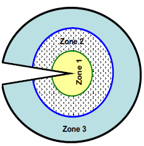
\includegraphics{Figures/Crack_zones}
	\decoRule
	\caption[Crack zones]{Names of each part of the crack}
	\label{fig:Fig4}
\end{figure}

The second zone, visible on \ref{fig:Fig4} is called singular zone: it circled the first zone. The mechanical field does not depend on specimen geometry. Interface between zone one and two, has continuous constraints and displacements values.

The last zone is the farthest zone from the crack tip. It is the zone which is in contact with loads and displacements forces.

As presented in \label{subsection}

%-----------------------------------
%	SUBSECTION 2
%-----------------------------------
\subsection{Mechanical field}

There are 2 mechanical fields, isotropic and orthotropic fields. Because of wood behavior, the orthotropic mechanical filed will be the only one presented. 
The elastic stress field, near the crack tip, depends on the material. For an orthotropic material, the expression, presented in \parencite{Reference10} work are :

\begin{equation}
	\left\{
	\begin{array}{rcr}
		\sigma_{11}=\frac{K_{1}}{(\sqrt{2 \pi r})}Re[\frac{s_{1}s_{2}}{(s_{1}-s_{2})}(\frac{s_{2}}{\sqrt{\rho_{2}}}-\frac{s_{1}}{\sqrt{\rho_{2}}})]+\frac{K_{2}}{(\sqrt{2 \pi r})}Re[\frac{1}{(s_{1}-s_{2})}(\frac{s_{2}^{2}}{\sqrt{\rho_{2}}}-\frac{s_{1}^{2}}{\sqrt{\rho_{1}}})]\\
		\sigma_{22}=\frac{K_{1}}{(\sqrt{2 \pi r})}Re[\frac{1}{s_{1}-s_{2}}(\frac{s_{1}}{\sqrt{\rho_{2}}}-\frac{s_{2}}{\sqrt{\rho_{1}}})]+\frac{K_{2}}{(\sqrt{2 \pi r})}Re[\frac{1}{(s_{1}-s_{2})}(\frac{1}{\sqrt{\rho_{2}}}-\frac{s_{1}}{\sqrt{\rho_{1}}})]\\
		\sigma_{21}=\sigma_{12}=\frac{K_{1}}{(\sqrt{2 \pi r})}Re[\frac{s_{1}s_{2}}{(s_{1}-s_{2}}(\frac{s_{1}}{\sqrt{\rho_{1}}}-\frac{1}{\sqrt{\rho_{2}}})]+\frac{K_{2}}{(\sqrt{ 2\pi r})}Re[\frac{1}{(s_{1}-s_{2})}(\frac{s_{1}}{\sqrt{\rho_{2}}}-\frac{s_{2}}{\sqrt{\rho_{1}}})] \\
	\end{array}
	\right.			
	\label{eq:stresses terms from Orthotropic field}
\end{equation} 

In these equations presented in \ref{eq:stresses terms from Orthotropic field}, $S_{i}$ with i = {1;2} are the polynomial roots calculated by another equation, using the components of the stiffness tensor for an orthotropic symmetry. 
Therefore, terms
\begin{equation}	
	\rho_{j}=\cos{\theta}+i s_{j} \sin{\theta} and j\in{[1;2]}
	\label{eq:terms present in stress equations}
\end{equation}			
These theories, are already used, and the orthotropic equations will be those that will be used for wood experiments. Indeed, even if the resolution could be done by ourselves, there are nowadays, computer software, which allow us to spend less time resolving orthotropic equations. It is written in the software program, and run, until finding solutions.

%-----------------------------------
%	SUBSECTION 3
%-----------------------------------
\subsection{Coefficient of intensity}

K is a coefficient of intensity, and $K_{Ic}$, is the one for the opening mode. The "c" means that it is the critical value of this coefficient. As \parencite{Reference10} explains, by using Laplace Carson inverse on intensity coefficient, it is possible to obtain crack opening factors. Focusing on mode I, it is particularly interesting to understand how $K_{Ic}$ evolves. The stress intensity factor K can be obtained by using finite element analysis (for example, with a contour integral method for orthotropic materials). It is obtained with the initial crack length $a_{initial}$ linked to the crack length L : $\frac{a_{initial}}{L}$.
The stress intensity factor depends on the specimen geometry. The classic linear elastic fracture mechanics equation for intensity coefficient is presented in \ref{eq:Intensity factor}:
\begin{equation}
	K_{I}=\frac{P}{W\sqrt{L}}f\frac{a_{initial}}{L} 	
	\label{eq:Intensity factor}
\end{equation} 						
P : the force applied on the specimen 
W the thickness
L the crack length 
f the linear function which link the terms $a_{initial}$ and L in $\frac{a_{initial}}{L}$. 


%----------------------------------------------------------------------------------------
%	SUBSECTION 4
%----------------------------------------------------------------------------------------

\subsection{Energetic methods}

Different methods were created to work on rupture mechanics, called energetic methods. $G_{\theta}$ or $M_{\theta}$ which are defined on surface contours. J and $G_{\theta}$ are useful for pure shearing or opening tests, due to a global energetic operation. All the presented integral with a $\theta$ terms have an important difference. They are defined on a surface contour, which is easier to integrate. M-integral has two terms, depending on real or virtual displacements involving real and virtual constraints, which allow decoupling modes
A-integral is an independent integral which allows to consider the effect of thermo-hygro-mechanical loads in the cracking process. During the crack process, it uses temperatures data. As T-integral, it is similar to M-integral, and do not include the crack tip, which is a particular part of the crack (too many singularities).

In this work, the chosen method, which is created in a Python program to realise this work is the Rice Integral.

Rice Integral is presented as the next formula \ref{eq:J, Rice integral} :
\begin{equation}
	J=\int_{\Gamma}[F n_{1}-\sigma_{ij} n_{j} \frac{\delta u_{i}}{\delta x_{1}}]d\Gamma
	\label{eq:J, Rice integral}
\end{equation}  

The considered contour of this integral is curvilinear and is named $\Gamma$. It includes the crack tip while it is not the case of others energetic method. “F” is the force applied on each part of the crack tip. Then, “a” is still the length of the crack. “$n_i$“ are the normal vectors to the curvilinear contour $\Gamma_{i}$, and $\sigma$ is the strain used to obtain crack opening. 
There are better energetics methods. As $G_{\theta}$ or $M_{\theta}$ which are defined on surface contours. J and $G_{\theta}$ are useful for pure shearing opening, due to a global energetic operation. But J integral will also allows us to work on mode I case. Then we will also use the complacency methode to obtain the energy release rate.

%----------------------------------------------------------------------------------------
%	SUBSECTION 4
%----------------------------------------------------------------------------------------

\subsection{Method of the complacency}

Complacency is the characterizing quantity of material elasticity behaviour. An elasticity compliance corresponds to the inverse of material elastic modulus. Its unity is the $Pa^-1$.
Complacency method is used to determinate the crack resistance. 
The formula used to calculate this energy release rate is written on \ref{eq:Energy release rate equation}:
\begin{equation}
	G_{c}= \frac{F_{c}^2}{2b} (\frac{\Delta C}{\Delta a})_{d} 	
	\label{eq:Energy release rate equation}
\end{equation}  
With : 
$G_c$ the value of energy release rate (in J/m²)
$F_c$ the critical force which involves the crack (in N)
b the thickness of the specimen (in mm)
$\Delta C$ the complacency evolution (in $Pa^-1$)
$\Delta a$ the crack length evolution (in mm)
In this work, C is determined in forced displacement, by the division of U, which is the imposed displacement, by F, the applied force. It must be noted that to have an idea of the imposed displacement depending on time, some articles as \parencite{Reference7} or \parencite{reference15} allow to fix this displacement between 2mm/min until 5mm/min.

As explained in previous part, the specimen presenting a RL surface studied have a Tangential dimension for their thickness. It involves a dimension evolution of this parameter. So for each test at a different MC, the b parameter must be measured, in order to have a precise value of G. Compacency method is often used in mode I analysis. It was the way of study for works as \parencite{}

%----------------------------------------------------------------------------------------
%	SECTION 4
%----------------------------------------------------------------------------------------

\section{Wood experimentations linked to climatical conditions :}

%----------------------------------------------------------------------------------------
%	SECTION 4
%----------------------------------------------------------------------------------------

\subsection{DCB (Double Cantilever Beam) test}

According to the different article on this test, it appears that it is used mainly with WS and DCB sample. As \parencite{Reference11} presents, it is a method permitting to study the crack tip and then estimate crack length during the wedge split test procedure. Most of the time, it is used in addition of DIC methods. For those reasons, this test is one of the most interesting in the presented case of a mode I study. It uses the compliance method for crack length estimation. 
The test is simple, as it is visible on \ref{fig:Fig6} it consists of using two arms surrounding the specimen which is fixed to the press by metallic grips. The tested specimen must be adapted to the system, such as ARCAN one, proposed by \parencite{Reference6}. The efforts are applied by an electromechanical press, in this work, the MTS allow to obtain the force applied for a given displacement per second. The chosen grips are simpler than ARCAN ones and allow only mode one tests.
\begin{figure}[th]
	\centering
	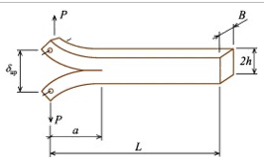
\includegraphics{Figures/DCB Test}
	\decoRule
	\caption[DCB Test]{Sheme of DCB Test in mode I, showing the different variables as $\delta_{ap}$, the opening length of the crack lips, a, the crack length, P the applied force and geometrical values of the specimen}
	\label{fig:Fig6}
\end{figure}
A sensor detects the movements of the application point of the forces.
Therefore, a camera is placed in the axis of the crack in order to use the images and study the crack.


%----------------------------------------------------------------------------------------
%	SUBSECTION 2
%----------------------------------------------------------------------------------------

\subsection{Climatical effects on the test}


This work studies the impact of temperature and moisture content variation on wood samples. The moisture content have an impact on the studied parameters as the energy rate or the mechanical resistance. Moreover, it is a phenomenon, present in the wild, which participate to wood life. Non precise technics allow to have an idea of the moisture content in the wood. But every specie is different and even, each tree is different. 
Without moisture meter the moisture content in our specimens is determined by the weight measurement of the sample. The concept is to dry the specimen to obtain the anhydrous weight. Thanks to this measure ($M_{0}$), and the actual weight ($M_{S}$) the \ref{eq:Moisture content depending on weight} is :
\begin{equation}
	H=\frac{_{M_{S}-M_{0}}}{M_{0}}100
	\label{eq:Moisture content depending on weight}
\end{equation} 

%----------------------------------------------------------------------------------------
%	SUBSECTION 3
%----------------------------------------------------------------------------------------

\section{Experiments on MMCG specimens depending on climatical conditions}

Research was already done on the subject, like \parencite{Reference12} studied on Jack pine (Pinus banksiana) and balsam poplar. He observes the mechanical properties of wood, function of the moisture content and temperature. It appears that another possibility to modify the moisture content, is the use of solution. \parencite{Reference12} presents three principal solutions, placed in a desiccator: MgCl2, NaNO3 and KCl. 

Another climatical condition which must be considered, is the temperature. The temperature can involve an augmentation of moisture content. Tests are done on this sample at normal temperature, but also at a lower one by putting specimen during 48 hours into a fridge. This experiment allows to prove the gain of moisture content due to the decreasing temperature. Scientists as \parencite{Reference13} did tests on sample under different temperature, 20\textcelsius, 40\textcelsius, 60\textcelsius and 80\textcelsius but also 100\textcelsius to 200\textcelsius during two hours for some DCB samples.
Tested samples were DCB ones and the species were Spruce and Beech. Results from works as \parencite{Reference12} on Balsam Poplar, but with compressive tests in a radial direction, allow to have an idea of the way to proceed and the attempt results. 

The last climatical conditions, presented is the fatigue load. Even if it is not a real climatical effect, it could be involved by the climate like a snow load. This is the last experiment which will be done on the specimen. Fatigue is directed by Paris law, as the \ref{eq:Paris law, fatigue loads equation} :
\begin{equation}
	\frac{\partial a}{\partial N}=C \Delta K^{m}
	\label{eq:Paris law, fatigue loads equation}
\end{equation} 
With “a”, the crack length, “N” the number of loading cycles, which involve that $\frac{\partial a}{\partial N}$ is the crack growth rate. It depends on the cyclic stress intensity factor $\Delta K$. Finally, “C” and “m” are empirical constants depending on the studied material, but also the frequency, the load ratio, the temperature... This equation allows to anticipate crack growth rate and predict fatigue comportment of the material. 

%----------------------------------------------------------------------------------------
%	SECTION 5
%----------------------------------------------------------------------------------------


\section{Test Results Analysis}

It is one of the principal digital measurement techniques using pictures. Digital Image Correlation (DIC) consists in comparing two images of the same object on load, as MMCG specimen in our case, and looking to the displacement field, in order to find a match between the two images. When a series of images is obtained, the comparison between these images, and their differences are analysed very accurately, pixel by pixel to obtain the real displacements, from one point to another place. The main problem of this technique is due to “noise” which involve uncertainties. Therefore, light problems can occur and decrease the precision of the results. In this method it is necessary to extract the two images (before and after movement).

%----------------------------------------------------------------------------------------
%	SUBSECTION 1
%----------------------------------------------------------------------------------------

\subsection{DIC Processus}


The DIC method is based on the principles of mechanical continuity (rigid body mechanics). The system consists of using a digital camera and specialised computer software, in this work, MatchID. Camera is used to capture consecutive images of the tested sample surface during the deformation test. Digital images determined by this way, which corresponds to a series of photos, is analysed by the DIC software. Displacement maps of specimen on the surface is created. Stress fields can be evaluated from strain fields. The formula used to obtain the displacement field is shown in \ref{eq:displacement field obtained by DIC methods}


\begin{equation}
	u^{k}=
	\begin{bmatrix}
		u_{z}^{k}\\u_{y}^{k}
	\end{bmatrix}
	=\Sigma^{N}_{i=1}
	\begin{bmatrix}
		f_{i}(k,\phi_{k}) & g_{i}(k,\phi_{k})\\ l_{i}(k,\phi_{k}) & m_{i}(k,\phi_{k})
	\end{bmatrix}
	\begin{bmatrix}
		A^{i}_{1}\\A^{i}_{2}
	\end{bmatrix}
	\begin{bmatrix}
		r^{i/2}_{k}
	\end{bmatrix}
	+
	\begin{bmatrix}
		T_{x}\\T_{y}
	\end{bmatrix}
	+
	R
	\begin{bmatrix}
		y_{k}\\y_{k}
	\end{bmatrix}
	\label{eq:displacement field obtained by DIC methods}
\end{equation} 
With $f_{i}$, $g_{i}$, $l_{i}$, $m_{i}$, polar functions, k is depending on the material because of Poisson term which determinates k. T terms are correction factors for rigid body motions.
Due to the fast and easy preparation, it is a very used fracture mechanic technique. After the determination of the displacement field, by using the integral method presented in last sections, it is possible to obtain the strain field.


%----------------------------------------------------------------------------------------
%	SUBSECTION 2
%----------------------------------------------------------------------------------------

\section{Examples on Wood}


If this method is used on wood, it is important to note that elastic orthotropic material model in 2D has five engineering constants as input parameters, to enter in the image analysis system. Even if it depends on the software used, these inputs are important to be known. First, Young modulus in longitudinal direction must be informed, $E_{L}$=$E_{1}$, transverse Young modulus $E_{trans}=E_{R}=E_{T}=E_{2}$. Then, shear modulus $G_{LR}=G_{LT}=G_{12}$, if shearing mode is studied. Therefore, Poisson coefficient $\nu$ has to be put into the software. This coefficient can change depending on the studied surface, in or out the plan. The initial crack length is introduced in the model. The damage description is presented by three principal inputs, even if it could change, depending on the software. Focusing on mode I damage, it is described by damage initiation stress $\sigma_{ini}$, but also separation at the failure $\delta_{fl}$, and exponential function shape coefficient $\alpha_{I}$. 

%----------------------------------------------------------------------------------------
%	SUBSECTION 3
%----------------------------------------------------------------------------------------

\subsection{Softwares and Match ID utilisations}

First it was decided to present one software for each method. Regarding the methods operation, it appears that they work with similar softwares. Indeed, as presented in last section, the method is always the analysis of two images and determining which are the differences. The only changes is the pattern on the sample, a grid, a marker, or the initial surface if it is not too uniform.
Aramis system develop software but also equipment to allow the best capture and resolution of images. It is used for DIC. 
Match ID will be the used software. 

\begin{figure}[th]
	\centering
	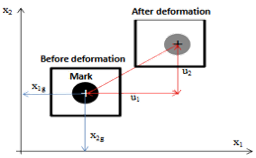
\includegraphics{Figures/Subset_Movement}
	\decoRule
	\caption[Subset Displacement]{Tracking markers scheme with the displacement of a mark before and after a deformation}
	\label{fig:Fig7}
\end{figure}

The MatchID software was chosen to compute DIC images and obtain displacement field and strain one. It is a powerful software with a new option which is linked to “crack” studies.
Thanks to this software, some ”.csv” files full of information were available. All the images recorded were treated with MatchID and every picture are divided into a large number of subsets. One subset is composed of 225pixels (square of 15 by 15 pixels). It is possible to have a look on the crack video, watch the different strains modelized by MatchID using every pixel’s evolution. Then the user must determine the initial length. Indeed, even if the specimens were manufactured with a precise shape, it was important to calibrate the initial length of the crack, by choosing the subset the closest to the crack tip.
When all these steps are done, for each experiment, so each specimen, a database have to be created. In these databases, will be found constant and information as this initial crack length $a_{0}$. Moreover, there is information, common to each test as the specimen geometry, filmed values or conversion factors.

As it is visible on \ref{fig:Fig7} DIC process works as Finit Element Method (FEM). Indeed a subset can be considered as an element of the project and then, looking to his displacement, strains and displacement map can be plot. The next section, will allow to better understand how a comparison between FEM and experiment can be done.


